\documentclass{article}
\usepackage[utf8]{inputenc}
\usepackage{amsmath}
\usepackage{amssymb}
\usepackage{graphicx}
\graphicspath{{Images/}}

\setlength{\oddsidemargin}{0in}
\setlength{\textwidth}{6.5in}
\setlength{\topmargin}{-.55in}
\setlength{\textheight}{9in}
\pagestyle{empty}


\title{Modern Algebra HW1}
\author{Michael Nameika}
\date{August 2022}

\begin{document}

\maketitle

\Large{\textbf{Section 2 Problems}}
\newline\newline
7. Is $*$ defined on $\mathbb{Q}$ by letting $a * b = a - b$ commutative? Associative? 
\newline
I claim that $*$ is neither associative nor commutative. To see $*$ is not commutative, let $a = 1, b = 2$ and note that
\[a * b = 1 - 2 = -1\]
and
\[b * a = 2 - 1 = 1 \neq a * b\]
To see $*$ is not associative, let $a = 5, b=c=1$ and consider
\[a* (b * c) = a * (1 - 1) = 5 * 0 = 5 - 0 = 5\]
and now consider
\[(a * b) * c = (5 - 1) * 1 = 4 - 1 = 3 \neq a * (b * c)\]
\newline\newline
9. Is $*$ defined on $\mathbb{Q}$ by letting $a * b = ab/2$ commutative? Associative?
\newline
I claim that $*$ is both associative and commutative. 
\newline
Proof: Let $a,b,c \in \mathbb{Q}$ and first consider $a * b$. By definition of $*$,
\[a * b = ab/2\]
and by commutativity of multiplication on $\mathbb{Q}$,
\[ab/2 = ba/2\]
by definition of $*$,
\[ba/2 = b * a\]
That is,
\[a * b = b * a\]
So $*$ is commutative. We now wish to show that $*$ is associative. First consider
\[a * (b * c) = a * (bc/2) = a(bc/2)/2\]
by associativity of multiplication on $\mathbb{Q}$, we find
\[a(bc/2)/2 = (ab/2)c/2 = (a * b) * c\]
Thus, $*$ is associative.
\newline\newline

\Large{\textbf{Section 2 Extra Problems}}
\newline
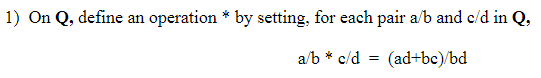
\includegraphics[]{extra problem1.PNG}
\newline

\includegraphics[]{well defined.PNG}
\newline\newline

I claim that $*$ is well-defined. Let $a/b, c/d \in \mathbb{Q}$ and suppose that $a/b$ can also be represented by $a'/b'$, and that $c/d$ can be similarly represented by $c'/d'$. We wish to show that $a/b * c/d$ and $a'/b' * c'/d'$ represent the same value.
To begin, by definition of $*$,
\[a/b * c/d = (ad + bc)/bd\]
and
\[a'/b' * c'/d' = (a'd' + b'c')/b'd'\]
To show these represent the same value, we must show that $(ad + bc)b'd' = (a'd' + b'c')bd$. Let us first compute the left hand side:
\[(ad + bc)b'd' = adb'd' + bcb'd'\]
by commutativity of multiplication on $\mathbb{Q}$,
\[ = ab'(dd') + cd'(bb')\]
and since $a/b$ and $a'/b'$ represent the same value, we have that $ab' = a'b$. Similarly for $c/d$ and $c'/d'$, we have $cd' = c'd$.
Substituting these into the above equation, we find
\[ab'(dd') + cd'(bb') = a'b(dd') + c'd(bb')\]
Factoring out $bd$, we get
\[a'b(dd') + c'd(bb') = (a'd' + c'b')(bd)\]
finally, we have
\[(ad + bc)b'd' = (a'd' + b'c')bd\]
So $*$ is well defined.


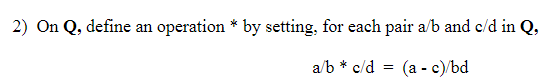
\includegraphics[]{extra problem 2.PNG}
\newline

\includegraphics[]{well defined.PNG}
\newline\newline

I claim that $*$ is not well-defined. To see this, let $a/b = 1/2$, $c/d = 2/3$ and note that
\[a/b * c/d = 1/2 * 2/3 = (1 - 2)/6 = -1/6\]
Notice that $1/2$ can also be represented as $2/4$, and now note
\[2/4 * 2/3 = (2-2)/12 = 0/12 = 0 \neq -1/6\]
That is, $*$ is not well-defined.
\newline\newline

\Large{\textbf{Section 4 Problems}}
\newline

2. Let $*$ be defined on $2\mathbb{Z} = \{2n \: | \: n \in \mathbb{Z}\}$ by letting $a * b = a + b$. Does $*$ give a group structure on $2\mathbb{Z}$?
\newline
I claim $\langle 2\mathbb{Z}, * \rangle$ forms a group. 
\newline
Proof: Let $a, b, c \in 2\mathbb{Z}$. We must first show associativity holds. Consider $a * (b * c)$:
\[a * (b * c) = a * (b + c) = a + (b + c)\]
by associativity of addition, 
\[a + ( b + c) = (a + b) + c\]
by definition of $*$,
\[ = (a * b) * c\]
So $*$ is associative.
\newline
I claim that $e = 0$ is the identity element of $\langle 2\mathbb{Z}, * \rangle$. Note that $n = 0 \in \mathbb{Z}$ and that $2n = 2\times 0 = 0 \in 2\mathbb{Z}$. Now consider $a * e$ and $e * a$:
\[a * e = a + 0 = a\]
\[e * a = 0 + a = a = a * e\]
So $*$ has an identity element, namely $e = 0$.
\newline
Now, for any $a \in 2\mathbb{Z}$, $a^{-1} = -a \in 2\mathbb{Z}$ since
\[a * a^{-1} = a + (-a) = 0 = e\]
and
\[a^{-1} * a = -a + a = 0 = e = a * a^{-1}\]
So each element has an inverse. Since $*$ is associative, has an identity element, and each $a \in 2\mathbb{Z}$ has an inverse under $*$, $\langle 2\mathbb{Z}, * \rangle$ forms a group.
\newline\newline
4. Let $*$ be defined on $\mathbb{Q}$ by letting $a * b = ab$. Does $*$ give a group structure on $\mathbb{Q}$?
\newline
I claim that $\langle \mathbb{Q}, * \rangle$ forms a group. 
\newline
Proof: Let $a, b, c \in \mathbb{Q}$ and first consider $a * (b * c)$:
\[a * (b * c) = a * (bc) = abc\]
By associativity of multiplication on $\mathbb{Q}$:
\[abc = (ab)c\]
\[ = (ab) * c\]
\[ = (a * b) * c\]
So $*$ is associative.
\newline
I claim the identity element is given by $e = 1$. Quickly note that $1 \in \mathbb{Q}$ and that
\[a * e = a\times 1 = a\]
\[e * a = 1 \times a = a = a * e\]
So $*$ has an identity element.
\newline
Finally, I claim that $*$ has an inverse for each element $a \in \mathbb{Q}$ and that the inverse is given by $a^{-1} = 1/a$. Notice that since $a \in \mathbb{Q}$, there exist $m \in \mathbb{Z}, n \in \mathbb{N}$ such that $a = m/n$. Then $1/a = 1/(m/n) = n/m \in \mathbb{Q}$. Additionally,
\[a * a^{-1} = a( 1/a) = 1 = e\]
\[a^{-1} * a = 1/a(a) = 1 = e = a * a^{-1}\]
So $*$ has an identity element for each $a \in \mathbb{Q}$. Thus, $\langle \mathbb{Q}, * \rangle$ forms a group.
\newline\newline
18. Determine if the following is a group: All $n \times n$ matrices with determinant either 1 or $-1$ under matrix multiplication.
\newline

Denote the set of all $n \times n$ matrices with determinant either $1$ or $-1$ by $D_{\pm 1}$. I claim that $\langle D_{\pm 1}, * \rangle$ forms a group where $*$ is standard matrix multiplication.
\newline
Proof: To begin, we must show that $D_{\pm 1}$ is closed under matrix multiplication. Let $M, N \in D_{\pm 1}$ and that, by determinant properties,  
\[\text{det}(MN) = \text{det}(M) \text{det}(N)\]
\[ = (\pm 1) (\pm 1)\]
\[ = \pm 1\]
So $MN \in D_{\pm 1}$. So we have that $*$ defines a binary operation on $D_1$. Now we must show that associativity holds.
Let $M, N, K \in D_{\pm 1}$ and consider
\[M * (N * K) = M * (NK) = MNK\]
By associativity of matrix multiplication,
\[MNK = (MN)K = (MN) * K = (M * N) * K\]
So associativity holds.
\newline
I claim that there exists an identity element, namely $e = I_n$ where $I_n$ is an $n \times n$ diagonal matrix of ones. Note that $\text{det}(I_n) = 1$, so $I_n \in D_{\pm 1}$. Notice
\[M * I_n = M(I_n) = M\]
\[I_n * M = I_n(M) = M = M * I_n\]
So $*$ has an identity element on $D_{\pm 1}$. Finally, I claim that for any $M \in D_{\pm 1}$, its inverse element is $M^{-1}$ where $M^{-1}$ denotes the standard matrix inverse. Recall that a square matrix $M$ is invertible if and only if $\text{det}(M) \neq 0$. For any $M \in D_{\pm 1}$, $\text{det}(M) = \pm 1$, so $M$ is invertible. Now notice
\[M * M^{-1} = MM^{-1} = I_n\]
\[M^{-1} * M = M^{-1}M = I_n = M * M^{-1}\]
That is, each $M \in D_{\pm 1}$ has an inverse under $*$. So $\langle D_{\pm 1}, * \rangle$ forms a group.
\end{document}
